\documentclass[12pt, a4wide]{scrreprt}

\usepackage{scrhack}
\usepackage{scrpage2}
\usepackage{graphicx}
\usepackage[utf8]{inputenc}
\usepackage{ngerman}
\usepackage{multicol}

\usepackage{titlesec}

%numbers braucht man wohl für IEEEtranN...
\usepackage[numbers]{natbib}

\begin{document}
\setkomafont{disposition}{\normalcolor\bfseries}
%-------Titelseite-------%
\noindent
Konstantin Obermann \hfill Mat.nr: 947545\\
Universität Osnabrück \hfill 23.10.2015\\
Wintersemester 15/16\\
\thispagestyle{empty}
\begin{center}

\includegraphics[scale=.9]{uos_proper.png}
\section*{}
{\LARGE Ausarbeitung zum Thema}\\
\section*{}
{\Huge {\bf Lokalisierung in drahtlosen Sensornetzwerken}}\\
\section*{}
{\Large Im Rahmen des Seminars ''Verteilte Systeme''}\\
\section*{}
{\Large Betreuer:}\\
{\Large Prof.Dr.rer.nat Nils Aschenbruck}\\
{\Large Dipl.-Inform. Matthias Schwamborn}\\
\end{center}

%-------Zusammenfassung-------%
\pagenumbering{roman}
\tableofcontents
\addcontentsline{toc}{chapter}{Einleitung und Motivation}

%-------Einleitung-------%
\pagenumbering{arabic}
\chapter{Einleitung und Motivation}
Der technologische und wirtschaftliche Fortschritt erfordert eine zuverlässige, konsistente und in vielen Fällen eine drahtlose Kommunikation. Die wohl bekanntesten drahtlosen Netzwerke sind die Mobilfunknetzstandards (GSM, UMTS, LTE), das WLAN und die WSN.\\
\indent 
Diese Ausarbeitung beschäftigt sich hauptsächlich mit den {\bf W}ireless {\bf S}ensor {\bf N}etworks (WSN). Die Lokalisierung der einzelnen Sensorknoten innerhalb WSNs erfolgt auf Basis von AOA, RSS oder distanzbasierten Ansätzen zur Positionsbestimmung. Eine schnelle Lokalisierung der einzelnen Sensoren erfolgt dann, wenn diese vorher optimal plaziert werden, um die Anzahl an Knoten im WSN zu minimieren und den Overhead in den Lokalisierungsalgorithmen zu vermeiden\cite{anchor_placement}.\\
\indent
Faktoren, wie Schnelligkeit und Präzision der Lokalisierung sowie der Grad der Autonomie des WSN, beeinflussen dessen Zuverlässigkeit und Potential. Dieses Potential ist entscheidend für die Auswahl an Einsatzmöglichkeiten eines WSN. Das Erdbeben-Frühwarnsystem (EEW) ist eines der Einsatzmöglichkeiten. Hier ist eine reibungslose und schnelle Kommunikation zwischen den Knoten besonders wichtig, denn ein Fehlalarm ist kostspielig. Allerdings ein im Ernstfall verspäteter Alarm kann Menschenleben kosten. Weitere Beispiele für die Verwendung von Sensornetzen sind Erkennung von Waldbränden, Überwachung von Deichen, Überwachung von Gebäudestatik, um Erdbebenschäden zu erkennen\cite{building_monitoring} oder das ''Precision Farming''. Bei dem letzten Beispiel werden Sensorknoten auf einem Landwirtschaftlich genutzten Feld verteilt, damit sie die Luftfeuchtigkeit, Temperatur, Grundwasserspiegel messen können. Diese Messungen sollen die Produktivität der Ernte steigern.\\
\indent
Zusätzlich zu den auftretenden Messfehlern treten natürliche Störfaktoren auf, die ein Problem darstellen und eine wichtige Rolle bei der Entwicklung und Optimierung dieser Lokalisierungstechniken spielen.

\chapter{Wireless Sensor Networks: Die Grundlagen}
Erstmalig wurde das Konzept des Sensornetzwerks in den 80\textit{er} Jahren für das Militär entwickelt, findet aber heute nach und nach mehr Anwendungsgebiete und, wie oben bereits erwähnt, vor allem im zivilen Einsatz.\\
\indent
Die WSNs bestehen aus vielen, nicht besonders leistungsstarken Sensoren, welche als Knoten (engl. nodes) in dem WSN dienen.
Diese Knoten sollen möglichst ohne externe Stromversorgung auskommen und können deshalb mit Batterien ausgestattet werden. Die Auswahl der Batterien hängt von der Zugänglichkeit der Knoten ab. Bei leicht erreichbaren und wartbaren Knoten eignen sich handelsübliche Batterien, wie z.B. die \textit{Energizer Ultra+}, welche bei 100\%\textit{iger} Auslastung des Knotensystems eine Laufzeit von bis zu 100 Stunden erreichen kann und bis zu 200 Stunden im Betrieb bleiben kann, wenn der Knoten nur zu 25\% der Zeit aktiv ist (also auch mal in Standbymodus geht)\cite{lifetime_study}.\\
\indent
Ein WSN mit nicht so schnell erreichbaren Knoten sollte mit leistungsstärkeren Batterien ausgestattet werden, wie zum Beispiel die von Tadiran\footnote{Französischer Hersteller für Lithiumbatterien (ehem. \textit{Sonnenschein Lithium})} hergestellte $LiSOCl_2$, welche in der Theorie eine Lebensdauer von bis zu 40 Jahre erreichen kann.\\
\indent
Bei den Knoten im WSN unterscheidet man zwischen \textit{Ankerknoten} bzw. \textit{Anker}, deren absolute Position initial bekannt ist und den \textit{Sensorknoten}, deren Position mithilfe der Anker bestimmt werden soll. 
Die weitere Ausstattung und somit die Kosten und Komplexität der Sensoren hängt von der Lokalisierungsmethode ab.\\
\indent
Einige Anwendungsbereiche erfordern einen zentralen Rechner. In diesem Fall sollte also ein- oder mehrere Knoten als Gateway konfiguriert werden, um klar definierte Schnittstelle(n) zur Zentrale zu bilden.\\
\indent
Zwar kann die Position der Knoten mit dem GPS ermittelt werden, allerdings erfordert die Vielseitigkeit der Einsatzmöglichkeiten der WSN eine Unabhängigkeit von der GPS-Positionierung. Das liegt daran, dass das GPS trotz der genauen Ortung ein zu schwaches Funksignal nutzt, welches eine zuverlässige  Ortung innerhalb von Gebäuden oder unter der Erde nicht möglich macht. Deswegen muss ein WSN in der Lage sein, eigenständig ein Netz zu initialisieren, alle Nichtanker-Knoten zu orten und ggf. deren Standortinformationen an einen zentralen Rechner weiterzugeben.

%\chapter{Die richtige Ankerplazierung}
%Die richtige Plazierung der Anker spielt eine große Rolle bei den meisten %Lokalisierungsmethoden.

\chapter{Ansätze zur Positionsbestimmung}
Die Hardware der Sensorknoten muss also den Umständen der Anwendungsbereiche angepasst werden. Da die Sensorausstattung ebenso von der Lokalisierungsmethode abhängt, hat die Wahl des passenden Ansatzes einen großen Einfluss auf die Kosten und den Energieverbrauch der Sensoren. Die Ansätze lassen sich in zwei grobe Kategorien einteilen.\\
\indent
Die erste Kategorie umfasst die \textit{range-based} Methoden, welche mit Abstands- oder Winkelmessung arbeiten. Diese nutzen die im weiteren Verlauf beschriebenen Ansätze wie AOA, TOA, TDoA, RSS und erreichen, auf Kosten von Komplexität, eine höhere Genauigkeit als die zweite Kategorie.\\
\indent
In die zweite Kategorie fallen die \textit{range-free} Methoden, also Lokalisierungstechniken, die auf einen direkten Bezug zwischen eines Ankers und eines Sensorknotens verzichten. Hierbei gibt es unterschiedliche Methoden und eine davon ist \textit{area-based}\cite{area_based}. Das Prinzip hierbei ist, dass die Anker mithilfe von unterschiedlich empfangenen Signalstärken untereinander eine Fläche generieren, in welcher sich der Sender befinden soll.\\
\indent
Die range-based Methoden eignen sich für WSNs, bei denen eine möglichst exakte Positionsbestimmung wichtig ist. Die range-free Lokalisierung ist eine Alternative, wenn die Ausstattung der Knoten im WSN möglichst kosteneffizient sein soll und die Kenntnis über die exakte Position der Sender nicht zwingend erforderlich ist.\\ 
\indent
Im Folgenden werden die im Fokus der Forschung liegenden Ansätze zur Positionsbestimmung vorgestellt.
  \section{Angle Of Arrival Ansätze}
Das Prinzip der {\bf A}ngle {\bf O}f {\bf A}rrival (AOA) Lokalisierung arbeitet mit dem Eintrittswinkel des empfangenen Signals. Dazu sollte der Empfänger einen ungehinderten Sichtkontakt zum Sender haben. Diese Lokalisierungsart kann in zwei Vorgehensweisen aufgeteilt werden, die in den Folgenden zwei Kapiteln beschrieben werden.
\newpage    
    \subsection{Das Beamforming Prinzip}
Beim Beamforming wird mithilfe einer Richtanenne ein ankommendes Signal normiert, indem der Empfangskegel der Richtanenne mechanisch oder elektronisch gedreht wird, bis das empfangene Signal die höchste Sendeleistung erreicht. Somit kann die Richtung des Senders bestimmt werden. Eine variierende Signalstärke ist ein Störfaktor bei dieser Methodik. Ein Ansatz, welcher in \cite{q1} besprochen wird, befasst sich mit mehreren rotierbaren Richtantennen, deren gesammelten Informationen durch eine Zentrale Einheit überlappt berechnet werden und somit eine höhere Genauigkeit erreicht werden. Laut \cite{q1} können mit 4 Richtantennen eine Richtungsgenauigkeit von $10^\circ -15^\circ$, mit 6 Antennen $5^\circ$ und mit bereits 8 Antennen eine Genauigkeit von $2^\circ$ erreicht werden.
    \subsection{Phase Interferometry}
Bei dem sog. \textit{phase interferometry}\cite{q1} Verfahren handelt es sich um die Bestimmung des eingehenden Signals durch eine Antennenfront. In {\bf Abb.3.1} ist der Aufbau skizziert. Hierbei sind $x1...xn$ die Antennen, welche mit dem gleichen Abstand $d$, welcher vorher bekannt ist, zueinander aufgebaut sind. Diese Antennen empfangen das Signal des Senders zu unterschiedlichen Zeitpunkten. Während die letzte Welle in diesem Beispiel gerade noch $x1$ verlässt, so tritt sie gleichzeitig bei $x2$ ein. Das ist der zeitliche Unterschied der empfangenen Phase, also die \textit{Phasenverschiebung}. Mithilfe dieses Phasenunterschiedes lässt sich mathematisch die Richtung des Senders bestimmen.\\

\begin{figure}[!htb]
\centering
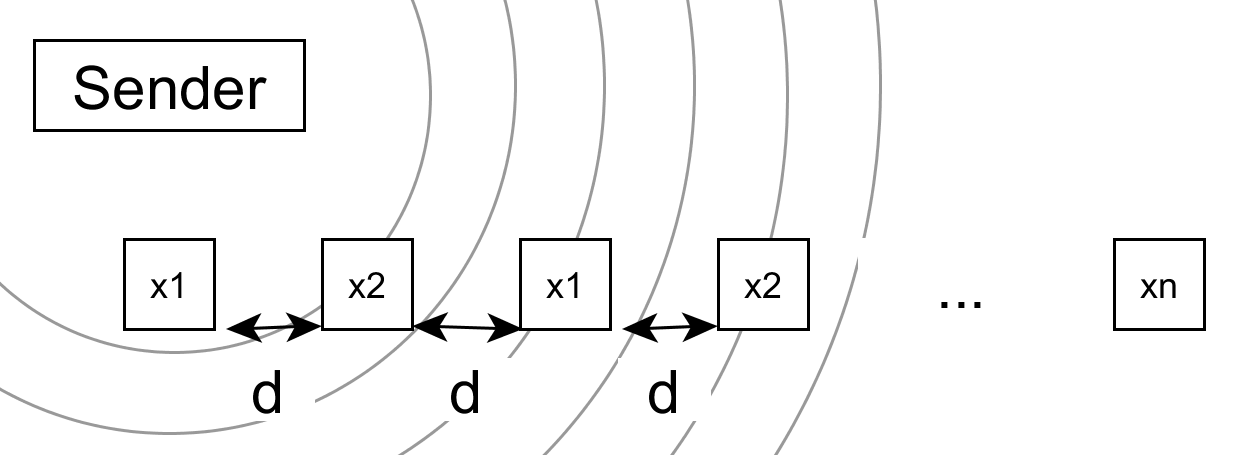
\includegraphics[scale=.3]{phase_int2.png}
\caption{Ankommende Wellenfronten an den Antennen}

\end{figure}
\newpage
  \section{Distanzbasierte Ansätze}
Bei den distanzbasierten Ansätzen werden zur Positionserkennung des Senders Informationen genutzt, welche fest mit dem Abstand zur Signalquelle korrelieren. Die Übertragungszeit eines Signals vom Sender zum Empfänger ist eine Information, welche genutzt werden kann, sowie die Übertragungs- und Rückkehrzeit (auch \textit{ping} genannt).
    \subsection{Lighthouse Approach}
    \subsection{One-Way Propagation/TOA}
    \subsection{Time Difference Of Arrival/TDOA}
    \subsection{Round-Trip Propagation/ping}
    \subsection{RSS-basierte Lokalisierung}    
  \section{Flächenbasierte Lokalisierung}
\chapter{Einsatzmöglichkeiten}
  \section{Kommerzieller Einsatz}
  \section{Industrieller Einsatz}

\chapter{Aktuelle Probleme und Fragestellungen}
  \section{Multipath propagation}
  \section{Shadowing}

\chapter{Zusammenfassung}

\newpage
%\bibliographystyle{te}
\bibliographystyle{IEEEtranN}

\begin{multicols}{2}
\bibliography{sources}
\nocite{*}
\end{multicols}
\end{document}